\chapter{Recurrent Nets}
% Authors: Qintai Liu
% Lecture date: 3/11/2019

\section{Simple Recurrent Net}
\label{sec:SimpleRecNet}
% Authors: Qintai Liu
% Lecture date: 3/11/2019

RNN is designed to capture sequential information.
Some of the inputs of traditional neural network are independent of each other.
But in many tasks, the inputs are actually dependent of each other.
In order to predict what the next word is in a sentence, you better know which words appear before it.
Recurrent nets perform the same task for every element of a sequence, with the output being depended on the previous computations. 
RNNs can take advantage of information in arbitrarily long sequences theoretically, but in reality they are limited to capturing long-term dependencies.
Here is what a typical RNN looks like:\cref{fig:Simple RNN}

\begin{figure}[h]
    \centering
    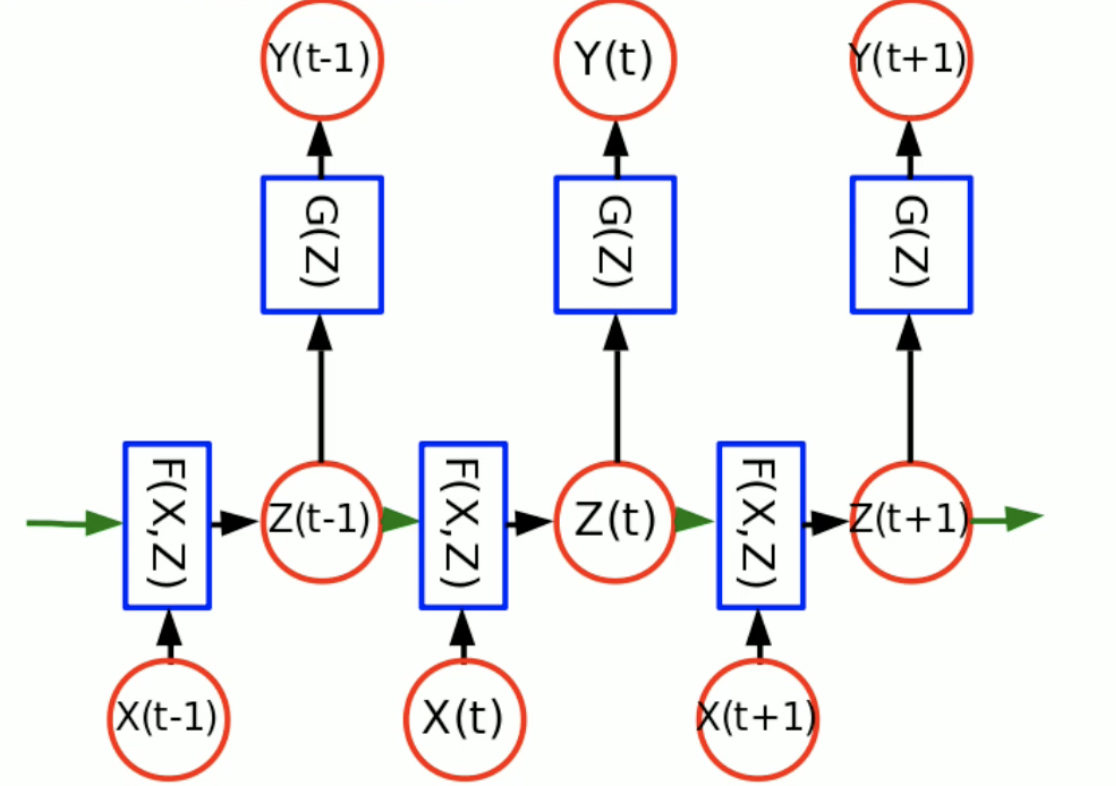
\includegraphics[width=150pt]{lectures/06-b/image/rnn.png}
    \caption{Simple Recurrent Net}
    \label{fig:Simple RNN}
\end{figure}

\begin{itemize}
  \item $\vect{x_{t}}$ is the input at time step $t$
  \item $\vect{z_{t}}$ is the hidden state at time $t$. $\vect{z_{t}}$ is calculated based on the input at the current step and the previous hidden state:
  $\vect{z_t} = F(\vect{x_t}, \vect{z_{t-1}})$
  \item $\vect{y_t}$ is the output at step $t$. $\vect{y_t} = G(\vect{z_t})$
\end{itemize}



\section{Issue of Simple Recurrent Net}
% Authors: Qintai Liu
% Lecture date: 3/11/2019
\subsection{Backpropagation Through Time}
% Authors: Qintai Liu
% Lecture date: 3/11/2019
In order to know the issue of simple RNN, we first need to know how the gradient is calculated in terms of RNN. Suppose the hidden state($\vect{z_t}$) is calculated as below:

\[\vect{\bar{z_t}} = \matr{W_X} \vect{x_t} + \matr{W_Z} \vect{z_{t-1}}\]
\[\vect{z_t} = f(\bar{\vect{z_t}})\]
\[\vect{y_t} = g(\vect{z_t})\]

To measures the effect of the $(t-n)$-th input symbot $x_{t-n}$, where $n\leq{t}$, on the $t$-th hidden state $\vect{z_t}$ of the simple recurrent neural network, we need to calculate the derivative shown below
\[\frac{\partial \vect{z_t}}{\partial \vect{x_{t-n}}}=\frac{\partial \vect{z_t}}{\partial \vect{z_{t-n}}}\frac{\partial \vect{z_{t-n}}}{\partial \vect{\bar{z}_{t-n}}}\frac{\partial \vect{\bar{z}_{t-n}}}{\partial \vect{x_{t-n}}}\]

Among these three terms in the right hand side of the above equation, we will focus on the first term

\begin{equation} \label{eq:bptt}
\frac{\partial \vect{z_t}}{\partial \vect{z_{t-n}}} = (\underbrace{\frac{\partial \vect{z_t}}{\partial \vect{\bar{z}_{t}}}}_{a}\underbrace{\frac{\partial \vect{\bar{z}_{t}}}{\partial \vect{z_{t-1}}}}_{b})
(\underbrace{\frac{\partial \vect{z_{t-1}}}{\partial \vect{\bar{z}_{t-1}}}}_{a}\underbrace{\frac{\partial \vect{\bar{z}_{t-1}}}{\partial \vect{z_{t-2}}}}_{b}) \ldots 
(\underbrace{\frac{\partial \vect{z_{t-n+1}}}{\partial \vect{\bar{z}_{t-n+1}}}}_{a}\underbrace{\frac{\partial \vect{\bar{z}_{t-n+1}}}{\partial \vect{z_{t-n}}}}_{b})
\end{equation}

First, consider \cref{eq:bptt}(a), which is the derivative of a nonlinear activation function used in the simple recurrent neural network.

Next, we look at \cref{eq:bptt}(b). We know

\[\frac{\partial \vect{\bar{z}_{t}}}{\partial \vect{z_{t-1}}} = \matr{W_Z}\]

From these two, we get
\begin{align} \label{eq:bptt_result}
\begin{split}
\frac{\partial \vect{z_t}}{\partial \vect{z_{t-n}}} &= (\frac{\partial \vect{z_t}}{\partial \vect{\bar{z}_{t}}}\frac{\partial \vect{\bar{z}_{t}}}{\partial \vect{z_{t-1}}})
(\frac{\partial \vect{z_{t-1}}}{\partial \vect{\bar{z}_{t-1}}}\frac{\partial \vect{\bar{z}_{t-1}}}{\partial \vect{z_{t-2}}}) \ldots 
(\frac{\partial \vect{z_{t-n+1}}}{\partial \vect{\bar{z}_{t-n+1}}}\frac{\partial \vect{\bar{z}_{t-n+1}}}{\partial \vect{z_{t-n}}}) \\
&= (\frac{\partial \vect{z_t}}{\partial \vect{\bar{z}_{t}}}\matr{W_Z})
(\frac{\partial \vect{z_{t-1}}}{\partial \vect{\bar{z}_{t-1}}}\matr{W_Z}) \ldots 
(\frac{\partial \vect{z_{t-n+1}}}{\partial \vect{\bar{z}_{t-n+1}}}\matr{W_Z}) \\
&= \prod\limits_{i=t-n+1}^{t} (\frac{\partial \vect{z_i}}{\partial \vect{\bar{z}_{i}}}\matr{W_Z})
\end{split}
\end{align}

Suppose the recurrent activation function $f$ is linear, \cref{eq:bptt_result} is reduced to
\begin{equation} \label{eq:bptt_linear_result}
\frac{\partial \vect{z_t}}{\partial \vect{z_{t-n}}} = \matr{W_Z}^{n-1}
\end{equation}


\subsection{Exploding Gradients}
% Authors: Qintai Liu
% Lecture date: 3/11/2019
When we do back-propagation in the recurrent neural networks, gradients of loss with respect to the weights can accumulate and result in very large gradients.
These in turn cause large updates to the neural network weights.

% In recurrent neural networks, gradients can accumulate during an update and result in very large gradients. 
% These in turn result in large updates to the network weights, and in turn, an unstable network. 

The explosion occurs through exponential growth by repeatedly multiplying gradients through the network layers that have values larger than $1.0$.

From \cref{eq:bptt_linear_result}, $\frac{\partial \vect{z_t}}{\partial \vect{z_{t-n}}}$ will likely explode as $n \rightarrow \inf$ if $e_{max} > 1$, where $e_{max}$ is the largest eigenvalue of $\matr{W_Z}$.

\subsection{Vanishing Gradients}
% Authors: Qintai Liu
% Lecture date: 3/11/2019
In recurrent neural networks, the gradients of loss with respect to the weights may also get smaller and smaller as we keep on moving backward in the network. 
In other words, the weights in the earlier layers get updated slowly compared with the neurons in the later layers.
These in turn result in a difficulty for training earlier layers of recurrent neural networks.

From \cref{eq:bptt_linear_result}, $\norm{\frac{\partial \vect{z_t}}{\partial \vect{z_{t-n}}}} \rightarrow 0$ when $e_{max} < 1$, where $e_{max}$ is the largest eigenvalue of $\matr{W_Z}$.

\section{Gradient clipping}
% Authors: Qintai Liu
% Lecture date: 3/11/2019
Fortunately it's easy to solve the problem of exploding gradients by doing gradient clipping \cite{1211.5063}.
First, in order to detect whether the exploding gradient arises, we could inspect the norm of the gradient of loss with respect to the parameters $\norm{\nabla}$.
If the gradient's norm is larger than some predefined threshold $\tau > 0$, we can renormalize the norm of the gradient to be $\tau$.

\[
\widetilde{\nabla}=\left\{
            \begin{array}{ll}
              \tau\frac{\nabla}{\norm{\nabla}} & \text{if}  \norm{\nabla}>\tau\\
              \nabla & \text{otherwise}
            \end{array}
          \right.
\]

\section{Long Short-Term Memory}
\label{sec:long-short-term-memory}
% Authors: Qintai Liu
% Lecture date: 3/11/2019


\begin{figure}[h]
  \centering
      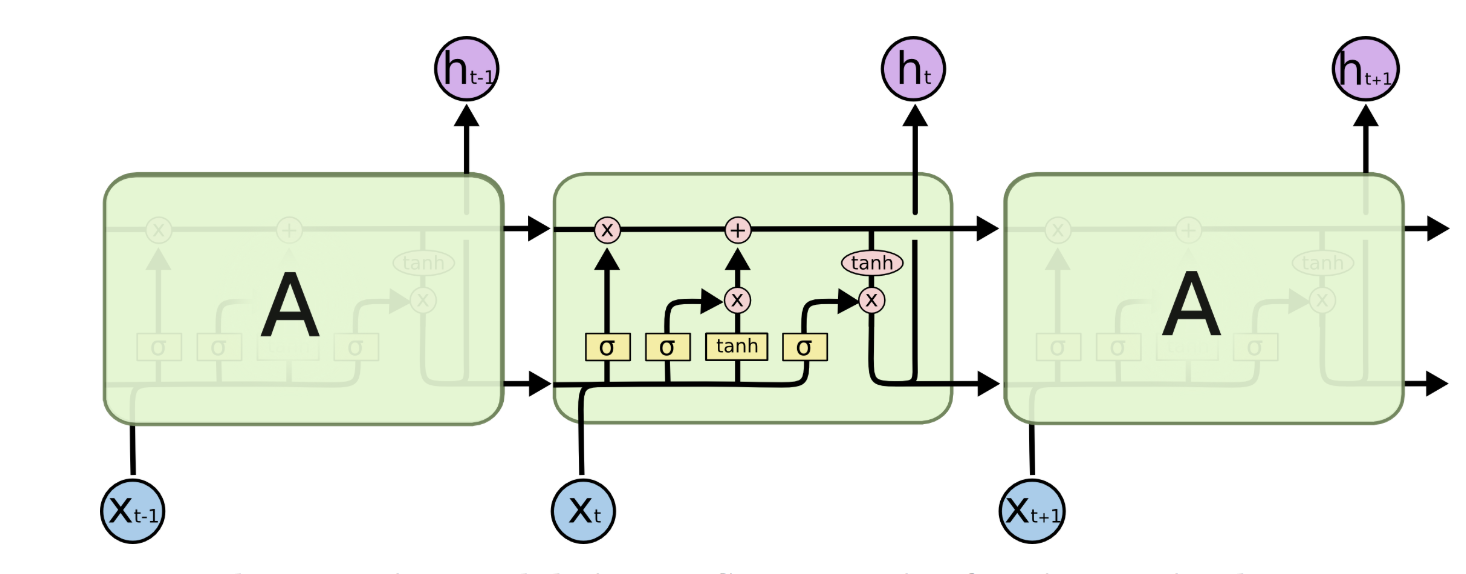
\includegraphics[width=0.8\textwidth,height=4.5cm]{lectures/06-b/image/lstm.png}
          \caption{
            The repeating module in an LSTM contains four interacting layers.
            \href{http://colah.github.io/posts/2015-08-Understanding-LSTMs/}{Source}
          }
          \label{fig:lstm}
\end{figure}

Long Short Term Memory networks \cite{article-lstm} are a special kind of RNN, capable of learning long-term dependencies. 
They work tremendously well on a large variety of problems, and are now widely used.
LSTMs are explicitly designed to avoid the long-term dependency problem. 
Below is how LSTM works

The forget gate in LSTM is to decide what information we’re going to throw away from the cell state.
\[\vect{f_t} = \sigma(\matr{W_{fh}}\vect{h_{t-1}}+\matr{W_{fx}}\vect{x_t} + \vect{b_f}) \]

Input gate decides which values we’ll update
\[\vect{i_t} = \sigma(\matr{W_{ih}}\vect{h_{t-1}} + \matr{W_{ix}}\vect{x_t} + \vect{b_i})\]

New candidate cell state is to decide what new information we’re going to store in the cell state.
\[\vect{\widetilde{c}_t} = tanh(\matr{W_{ch}}\vect{h_{t-1}} + \matr{W_{cx}}\vect{x_t} + \vect{b_c})\]

New cell state:
\[\vect{c_t} = \vect{f_t}*\vect{c_{t-1}} + \vect{i_t}*\vect{\widetilde{c}_t}\]

Output Gate decides what parts of the cell state we’re going to output.
\[\vect{o_t} = \sigma(\matr{W_{oh}}\vect{h_{t-1}} + \matr{W_{ox}}\vect{x_t} + \vect{b_o})\]

Output:
\[\vect{h_t} = \vect{o_t}*tanh\vect{(c_t)}\]

\section{Gated Recurrent Units}
% Authors: Qintai Liu
% Lecture date: 3/11/2019

\begin{figure}[h]
  \centering
      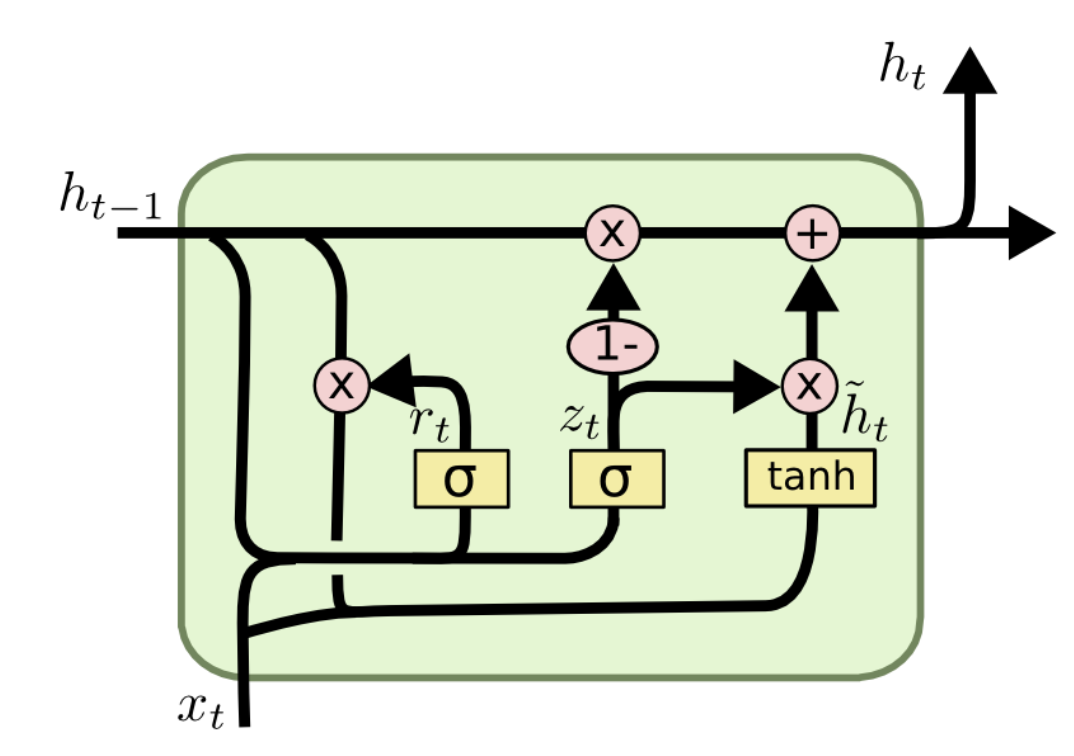
\includegraphics[width=0.5\textwidth,height=4.5cm]{lectures/06-b/image/GRU.png}
          \caption{
            Gated Recurrent Units
            \href{http://colah.github.io/posts/2015-08-Understanding-LSTMs/}{Source}
          }
          \label{fig:gru}
\end{figure}

A slightly more dramatic variation on the LSTM is the Gated Recurrent Unit \cite{1406.1078}.
It combines the forget and input gates into a single “update gate.” 
It also merges the cell state and hidden state, and makes some other changes. 
The resulting model is simpler than standard LSTM models.
Below is how GRU works

The update gate decides what information from the past would be passed to the next cell state.

\[\vect{z_t} = \sigma(\matr{W_{zh}}\vect{h_{t-1}}+\matr{W_{zx}}\vect{x_t} + \vect{b_z}) \]

The reset gate determine what information would be discarded from previous cell states.

\[\vect{r_t} = \sigma(\matr{W_{rh}}\vect{h_{t-1}}+\matr{W_{rx}}\vect{x_t} + \vect{b_r}) \]

Then the current memory content update the stories the latest important information by using the reset gate.

\[\vect{\widetilde{h}_t} = \tanh(\matr{W_{hr}}(\vect{r_t}*\vect{h_{t-1}}) + \matr{W_{hx}}\vect{x_t} + \vect{b_h})\]

Finally, the final cell state updates the information gained from the current unit and passed it to the next cell.

\[\vect{h_t} = (1-\vect{z_t})*\vect{h_{t-1}} + \vect{z_t}*\vect{\widetilde{h}_t}\]